%%%%%%%%%%%%%%%%%%%%%%%%%%%%%%%%%%%%%%%%%%%%%%%%%%%%%%%%%%%%%%%%%%%%%%%%%%%%%%%%%%%%%%%
%%%%%%%%%%%%%%%%%%%%%%%%%%%%%%%%%%%%%%%%%%%%%%%%%%%%%%%%%%%%%%%%%%%%%%%%%%%%%%%%%%%%%%%
% 
% This top part of the document is called the 'preamble'.  Modify it with caution!
%
% The real document starts below where it says 'The main document starts here'.

\documentclass[12pt]{article}
\usepackage{graphicx}
\usepackage{float}
\usepackage{amssymb,amsmath,amsthm}
\usepackage[top=1in, bottom=1in, left=1.25in, right=1.25in]{geometry}
\usepackage{fancyhdr}
\usepackage{enumerate}
\usepackage{listings}


% Comment the following line to use TeX's default font of Computer Modern.
\usepackage{times,txfonts}

\newtheoremstyle{homework}% name of the style to be used
  {18pt}% measure of space to leave above the theorem. E.g.: 3pt
  {12pt}% measure of space to leave below the theorem. E.g.: 3pt
  {}% name of font to use in the body of the theorem
  {}% measure of space to indent
  {\bfseries}% name of head font
  {:}% punctuation between head and body
  {2ex}% space after theorem head; " " = normal interword space
  {}% Manually specify head
\theoremstyle{homework} 

% Set up an Exercise environment and a Solution label.
\newtheorem*{exercisecore}{Exercise \@currentlabel}
\newenvironment{exercise}[1]
{\def\@currentlabel{#1}\exercisecore}
{\endexercisecore}

\newcommand{\localhead}[1]{\par\smallskip\noindent\textbf{#1}\nobreak\\}%
\newcommand\solution{\localhead{Solution:}}

%%%%%%%%%%%%%%%%%%%%%%%%%%%%%%%%%%%%%%%%%%%%%%%%%%%%%%%%%%%%%%%%%%%%%%%%
%
% Stuff for getting the name/document date/title across the header
\makeatletter
\RequirePackage{fancyhdr}
\pagestyle{fancy}
\fancyfoot[C]{\ifnum \value{page} > 1\relax\thepage\fi}
\fancyhead[L]{\ifx\@doclabel\@empty\else\@doclabel\fi}
\fancyhead[C]{\ifx\@docdate\@empty\else\@docdate\fi}
\fancyhead[R]{\ifx\@docauthor\@empty\else\@docauthor\fi}
\headheight 15pt

\def\doclabel#1{\gdef\@doclabel{#1}}
\doclabel{Use {\tt\textbackslash doclabel\{MY LABEL\}}.}
\def\docdate#1{\gdef\@docdate{#1}}
\docdate{Use {\tt\textbackslash docdate\{MY DATE\}}.}
\def\docauthor#1{\gdef\@docauthor{#1}}
\docauthor{Use {\tt\textbackslash docauthor\{MY NAME\}}.}
\makeatother

% Shortcuts for blackboard bold number sets (reals, integers, etc.)
\newcommand{\Reals}{\ensuremath{\mathbb R}}
\newcommand{\Nats}{\ensuremath{\mathbb N}}
\newcommand{\Ints}{\ensuremath{\mathbb Z}}
\newcommand{\Rats}{\ensuremath{\mathbb Q}}
\newcommand{\Cplx}{\ensuremath{\mathbb C}}
%% Some equivalents that some people may prefer.
\let\RR\Reals
\let\NN\Nats
\let\II\Ints
\let\CC\Cplx

%%%%%%%%%%%%%%%%%%%%%%%%%%%%%%%%%%%%%%%%%%%%%%%%%%%%%%%%%%%%%%%%%%%%%%%%%%%%%%%%%%%%%%%
%%%%%%%%%%%%%%%%%%%%%%%%%%%%%%%%%%%%%%%%%%%%%%%%%%%%%%%%%%%%%%%%%%%%%%%%%%%%%%%%%%%%%%%
% 
% The main document start here.

% The following commands set up the material that appears in the header.
\doclabel{Stat 300: Homework 5}
\docauthor{Stefano Fochesatto}
\docdate{\today}

\begin{document}


\hspace{.5in}\textbf{Exercise 3.82:} Consider writing into a computer disk and then sending\\

it through a certifier that counts the number of missing pulses. Suppose this number $X$ has a 
Poisson distribution with the parameter $\mu = .2$\\

\begin{enumerate}
  \item What is the probability that the disk has exaclty one missing pulse. \\
  
  \textbf{Answer:} Using the pmf for a Poissan distribution when $\mu = .2$ and $X = 1$.
\begin{equation*}
  P(X = 1) = p(1;.2) = \dfrac{e^{-.2}.2}{1} = .1637.
\end{equation*}
  \vspace{.25in}

  
  \item What is the probability that a disk has at least two missing pulses.\\
  
  \textbf{Answer:} The probability that the disk has at least two missing pulses is the same as
  1 - the probability the disk has at most 1 missing pulse. Therefore,
  \begin{equation*}
    P(X \geq 2) = 1 - P(X \le 1) = 1 - F(1;.02) = 1 - .982 = .018.
  \end{equation*}
  \vspace{.25in}

  
  \item If two disks are independently selected what is the probability that neither contains a missing pulse.\\
  
  \textbf{Answer:} First let's calculate the probability that the disk has no missing pulses,
  \begin{equation*}
    P(X = 0) = p(0,.2) = \dfrac{e^{-.2}}{1} =.819.
  \end{equation*}
  Since the drives are independent we simply multiply the probabilities, 
  \begin{equation*}
    P(X_1 \cap X_2) = .819^2 = .671.
  \end{equation*}
  \vspace{.5in}
\end{enumerate}











\hspace{.5in}\textbf{Exercise 4.2:} Suppose the reaction temperature $X$ 
$(in C)$ in a certain chemical process has a uniform distribution with  $A = -5$ and $B = 5$.\\
\begin{enumerate}
  
  
  
  
  \item Compute $P(X<0)$\\
  
  \textbf{Answer:} Since the $X$ has a uniform distribution,
  \begin{equation*}
    P(X<0) = P(-5\le X \le 0) = \dfrac{1}{10}(0 + 5) = .50.
  \end{equation*}
  \vspace{.25in}
  
  
  
  
  
  \item Compute $P(-2.5 < X < 2.5)$\\
  
  \textbf{Answer:} Again since $X$ has a uniform distribution over a support length 10,
  \begin{equation*}
    P(-2.5 < X < 2.5) = P(-2.5 \le X \le 2.5) = \dfrac{1}{10}(2.5 - (-2.5)) = .5
  \end{equation*}
  \vspace{.25in}
  
  
  
  \item Compute $P(-2 \le X \le 3)$\\
  
  \textbf{Answer:} 
  \begin{equation*}
    P(-2 \le X \le 3) = \dfrac{1}{10}(3 - (-2)) = .5
  \end{equation*}
  \vspace{.25in}
  
  
  
  \item For $k$ satisfying $-5<k<k+4<5$, compute $P(k<X<k+4)$\\
  
  \textbf{Answer:} 
  \begin{equation*}
    P(k<X<k+4) = P(k \le X \le k+4) = \dfrac{1}{10}(k + 4 - k) = .40. 
  \end{equation*}
  
\end{enumerate}

\vspace{.5in}




\hspace{.5in}\textbf{Exercise Extra:} 
\begin{enumerate}
  \item Find the mean and variance of the dates. What does this tell you about the distribution 
  of air accidents? (Hint: if they were Poisson,the mean and variance would be similar). Looking
   at the data, do you have a guess about the pattern?\\
  
  \textbf{Console:}
  \lstinputlisting{r.txt}

  \solution So we can see that the mean and median are relatively close, therefore there are not many outliers skewing the data.
  We can see that the mean, or expected value is nowhere close to the variance so its very Unlikely that this data is Poisson. looking at a histogram
  the data looks like a flat normal with a slight right skew. 




  \item Assuming the data was Poisson with mean 10.2, what is the probability of getting 
  exactly 27 accidents in a year? BONUS: What is the probability of getting 27 or more 
  accidents in a year? Does this tell you anything about the patterns of accidents?\\
  
  \solution We simply calculate, $P(X = 27)$, where $X \sim Poisson(10.2)$
  \begin{equation*}
    P(X = 27) = p(27;10.2) = \dfrac{e^{-10.2}10.2^{27}}{27!} = 5.826 \times 10^{-6}
  \end{equation*}


\end{enumerate} 
\vspace{.5in}










\hspace{.5in}\textbf{Exercise Extra:} If large earthquakes are a Poisson 
process with rate 2 per year, what is the probability that you get zero 
quakes in four years? What IS a Poisson process? Is it a reasonable model
 for earthquakes (why or why not?)\\


\solution Since we know that large earthquakes are a Poisson process that occur at a rate of 2 per year, in order
to calculate the probability that zero quakes occur over the span 4 years we need to calculate $\mu$ for our time interval and the 
evaluate $p(X = 0; \mu)$. Note that $\mu = mean = 4\cdot 2 = 8$. Thus calculating thr probability,
\begin{equation*}
  P(X = 0) = \dfrac{e^{-8}8^{0}}{0!} = 3.355 \times 10^4
\end{equation*}
The Poisson process is used to is used to model the occurrences of a certain event that appears to have a rate, but occirs completly at random. Event like earthquakes, accident in industrial facilities. Thud this is a reasonable model for earthquakes. 
\vspace{.5in}





\hspace{.5in}\textbf{Exercise 3.110:} Grasshoppers  are  distributed  at  random  in  a  large  field  according to a Poisson process with parameter $\alpha = 2$ per square yard. How large should the radius R of a circular sampling region be taken so that the probability of find-ing at least one in the region equals .99?\\

\solution 

First we star by using the pmf for the poisson process to calculate $\mu$ given that $P(X \geq 1) = .99$,
\begin{equation}
  .99 = P(X \geq 1) = 1 - P(X = 0) = 1 - \dfrac{e^{-\mu}\mu^0}{0!} = 1 - e^{-\mu}.
\end{equation}
Solving for $\mu$ we get,
\begin{equation*}
  \mu = -ln(.01).
\end{equation*}
Thus we know that the area $A$ of the field must be,
\begin{equation*}
  A = \dfrac{\mu}{\alpha} = \dfrac{\mu}{2} =  \dfrac{-ln(01)}{2}.
\end{equation*}
Solving for the radius, since $A = \pi R^2$,\\
\begin{equation*}
  R = \sqrt{\dfrac{-ln(01)}{\pi2}} = .8561.
\end{equation*}

\vspace{.5in}





\hspace{.5in}\textbf{Exercise 4.4:} Let $X$ denote the vibratory stress on a wind turbine
blade ar a particular wind speed in a wind tunnel, with pdf,
\center
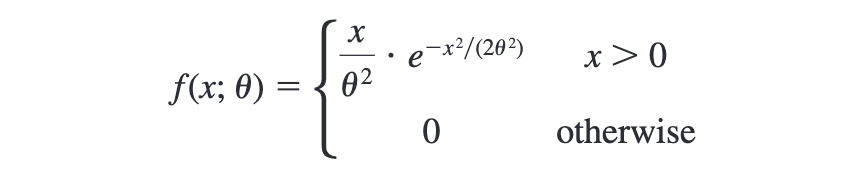
\includegraphics[width = \textwidth]{pdf.png}
\center


\begin{enumerate}
  \item Verify that $f(x;\theta)$ is a legitimate pdf\\
  
  \solution Integrating $f(x;\theta)$ over the support,
  \begin{equation*}
    \int_{0}^{\infty} \dfrac{x}{\theta^2}e^{\frac{-x^2}{2\theta^2}} = -e^{\frac{-x^2}{2\theta^2}} |_{0}^{\infty} = 0-(-1) = 1
  \end{equation*}
  This the given pdf is valid. 
  \vspace{.25in}


  \item Suppose $\theta = 100 $ (a  value  suggested  by  a  graph  in  the article). What is the probability that $X$ is at most 200? Less than 200? At least 200?\\
  
  \solution
  Since we had to solve for the cdf to find out if we have a valid pdf, we can compute all these probabilities by simply plugging in the values,
  \begin{equation*}
    P(X \le 200) = -e^{\frac{-x^2}{2(100)^2}} |_{0}^{200} = .8647
  \end{equation*}
  Since our variable is a continuos random variable,
  \begin{equation*}
    P(X < 200) = P(X \le 200) =  .8647.
  \end{equation*}
  \begin{equation*}
    P(X \geq 200) = 1 -  P(X < 200) = 1 - .8647 = .1353.
  \end{equation*}

\end{enumerate}
\vspace{.5in}


\hspace{.5in}\textbf{Exercise 4.10:} A  family  of  pdf’s  that  has  been  used  to  approximate 
 the  distribution  of  income,  city  population  size,  and  size  of 
 firms is the Pareto family. The family has two parameters, $k$ and $u$, both > 0, and the pdf is,
 \center
 
\includegraphics[width = \textwidth]{pdf1.png}
 \center
 \begin{enumerate}
   
   
   \item Sketch a graph of the pdf.\\
   
\solution I offer a sketch with my words, 
The graph is $f(x) = 0$ until $x = \theta$ then it looks like $f(x) = 1/x$ where $f(\theta) = \frac{k}{\theta}$. 
\vspace{.25in}


\item Verify that the total area under the graph equals 1.\\

\solution Integrating over the non-zero support,
\begin{align*}
  \int_{\theta}^{\infty} \dfrac{k\theta^k}{x^{k+1}} &=  k\theta^k \int_{\theta}^{\infty} \dfrac{1}{x^{k+1}}, \\
  &= x^{-k}|_\theta^{\infty}(-\theta^k), \\
  &=(0 - \theta^{-k}) (-\theta^k),\\
  &= 1.  
\end{align*}

\vspace{.25in}


\item Find the closed form for the cdf, for $b > \theta$.\\

\solution Using the pdf to solve for $P(X \le b)$,
\begin{align*}
  P(X \le b)\int_{\theta}^{b} \dfrac{k\theta^k}{x^{k+1}} &= k\theta^k \int_{\theta}^{b} \dfrac{1}{x^{k+1}},\\
  &= x^{-k}|_\theta^{b}(-\theta^k),\\
  &=(b^-k - \theta^{-k}) (-\theta^k).
\end{align*}

\vspace{.25in}


\item Find the closed form for the cdf, for $b > a >\theta$.\\

\solution Using the pdf to solve for $P(a \le X \le b)$,
\begin{align*}
  P(a \le X \le b)\int_{a}^{b} \dfrac{k\theta^k}{x^{k+1}} &= k\theta^k \int_{a}^{b} \dfrac{1}{x^{k+1}},\\
  &= x^{-k}|_a^{b}(-\theta^k),\\
  &=(b^-k - a^{-k}) (-\theta^k).
\end{align*}

 \end{enumerate}

 \vspace{.5in}









 \hspace{.5in}\textbf{Exercise 4.12:} The cdf for X (5 measurement error) of Exercise 3 is,
 \center
 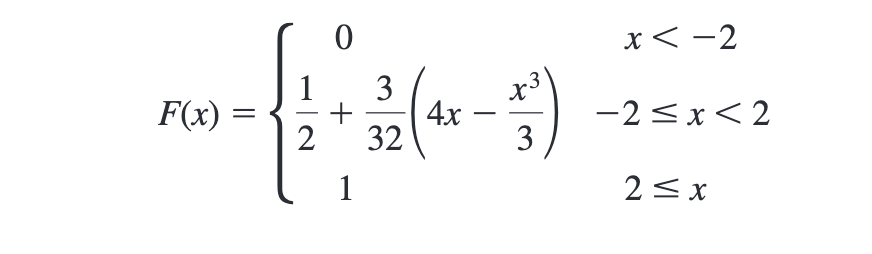
\includegraphics[width = \textwidth]{pdf2.png}
 \center
\begin{enumerate}
  \item Compute $P(X<0)$,
  \solution Plugging into the given cdf,
  \begin{equation*}
    P(X<0) = P(X \le 0) = F(0) = .5 .
  \end{equation*}
  \vspace{.25in}


  \item Compute $P(-1< X < 1)$,
  \solution Plugging into the given cdf,
  \begin{equation*}
    P(-1< X < 1) = P(X \le 1) - P(X \le -1)  = F(1) - F(-1) = \dfrac{11}{16} = .6875.
  \end{equation*}
  \vspace{.25in}



  \item Compute $P(.5 < X )$,
  \solution Plugging into the given cdf,
  \begin{equation*}
    P(.5 < X )= 1 - P(X \le .5)  = 1 - F(.5) = .3164.
  \end{equation*}
  \vspace{.25in}
\end{enumerate}











\hspace{.5in}\textbf{Exercise 4.22:} 
























\end{document}